	\chapter{Installation Notes}
\codetext{!\{sys.executable\} -m pip install pandas-profiling}

Use this to import from another directory.
	\begin{code}[\codenumbering]{}
		\codeitemnonumber import sys
		\codeitemnonumber sys.path.insert(1, "..\textbackslash{}lendres\textbackslash{}")
	\end{code}


Code folding:
https://jupyter-contrib-nbextensions.readthedocs.io/en/latest/install.html

\textcode{conda install -c conda-forge jupyter\_contrib\_nbextensions}
	\begin{figure}[tbp]
		\centering
		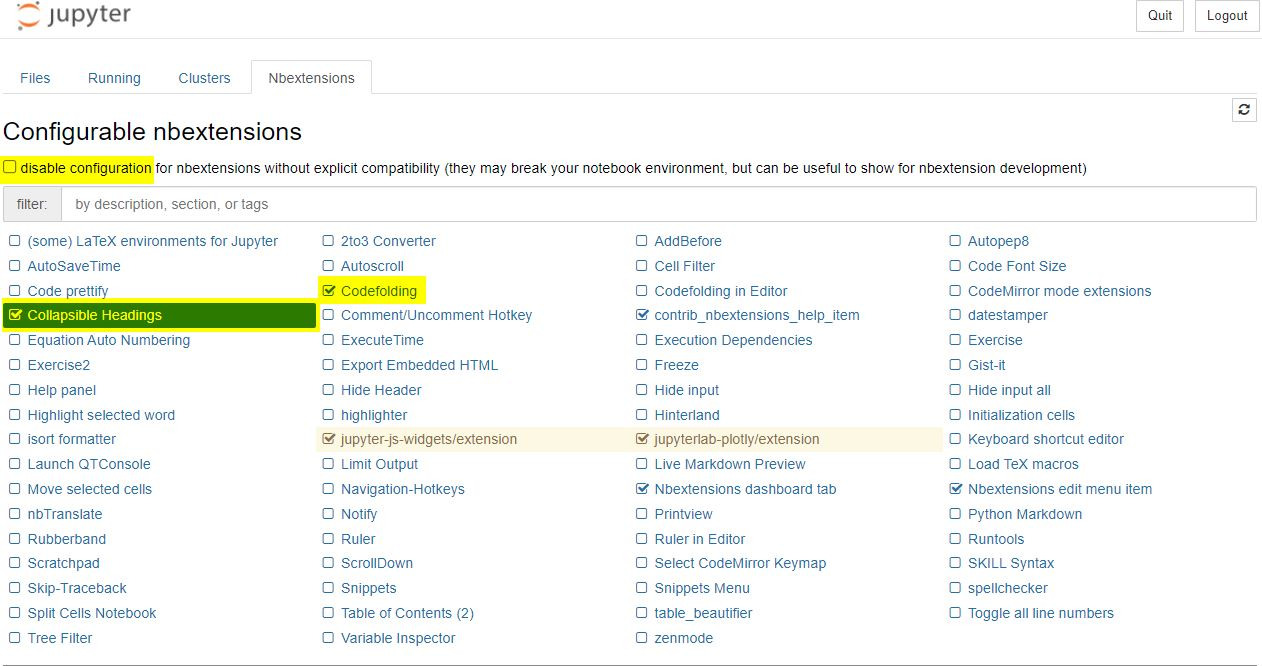
\includegraphics[width=\textwidth]{jupyterenablefolding}
		\caption{Enable nbextensions for Jupyter notebooks.}
		\label{fig:normaldistrution}
	\end{figure}


	\section{Imbalanced}
	\begin{code}[\codenumbering]{}
		\codeitemnonumber \# Jupyter notebook
		\codeitemnonumber !pip install imblearn --user
		\codeitemnonumber !pip install imbalanced-learn --user
		\codeitemnonumber
		\codeitemnonumber \# Anaconda prompt
		\codeitemnonumber \#!pip install -U imbalanced-learn

		\codeitemnonumber \#conda install -c conda-forge imbalanced-learn

		\codeitemnonumber \# Restart the kernel after successful installation of the library
	\end{code}

	\section{Anaconda and Python}
	\begin{code}[\codenumbering]{}
		\codeitemnonumber conda update -n base conda
		\codeitemnonumber conda update --all
		\codeitemnonumber jupyter contrib nbextension install --user
	\end{code}